\chapter{Implementation}
\section{Database} \label{Database}
\begin{figure}[h]
\centering
\frame{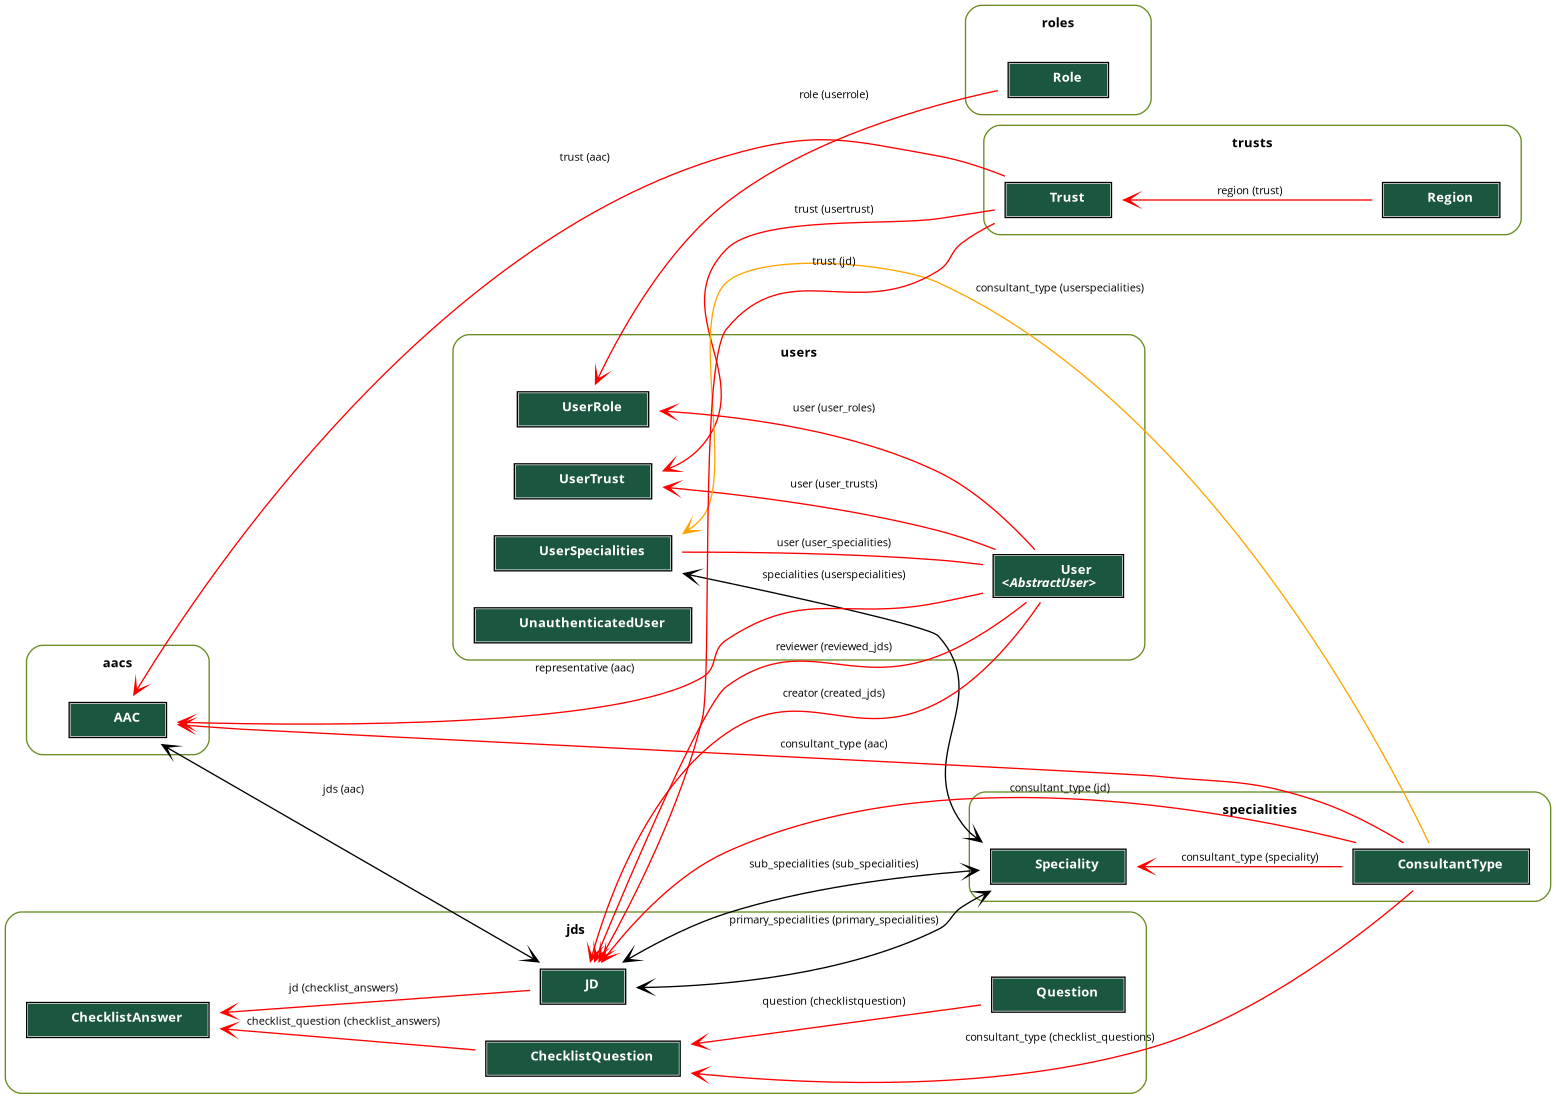
\includegraphics[width=\linewidth]{images/database.png}}
\vspace{-20pt}
\caption{Database schema without fields (backend/*/models.py)}
\label{fig:database}
\vspace{-5pt}
\end{figure}
Figure \ref{fig:database} represents the database schema. Due to the large number of models, fields have been omitted in this figure to maintain readability. See Appendix \ref{app:Database} for a full version. This diagram aptly presents just how intertwined this system is, as well as the sheet number of data taken into consideration during the process.

This relational database schema allows for handing of detailed user profiles, Job Descriptions (JDs), and Advisory Appointment Committees (AACs). It allows for a sophisticated access control system based on roles, Trust, and consultant types. 

Normalisation helps in organizing data efficiently and reduces the redundancy by ensuring that each data item is stored only once. For instance, separating user details from roles and trust levels allows for easy updates and management without unnecessary duplication. 

The clear definition of relationships between entities, such as one-to-many and many-to-many, is a manifestation of thoughtful consideration of how the models should relate to each other. It allows accurate, error-minimal and efficient querying of the database by using the minimum number of tables necessary. Foreign keys ensure that relationships between entities are consistent and that orphan records are avoided.

Separation of UserRole, UserTrust, and UserSpecialities is essential as users often have multiple roles and specialities. They may also be associated with different Trusts, which must be recorded to avoid conflicts of interest. A many-to-many relationship is not sufficient as each role and trust must be approved by an administrator first. We also need to ensure that users are not shown information from entities that they are approved for, but have not requested in the profile page. 

Specialities and Trusts also have hierarchical relationships. Consultant Types are associated with differing specialities, so JDs should not be allowed to contain both radiology and oncology specialities. Trusts fall into Regions, which are used to decide which RSA should be prioritised to review the JD.

As always, fields are give intuitive names, and the correct data types and constraints are used for data integrity. God tables are avoided entirely as large numbers of rows cause performance issues and increase complexity.

Without such a detailed schema, at best the system would be completely static. Policies change often, new Trusts join or are renamed, and specialities are added or removed. Without an extremely flexible database, this website would be unusable within a matter of months.

\section{API}
\subsection{Endpoints}
\begin{listing}[!ht]
\begin{minted}[
    frame=lines,
    framesep=2mm,
    fontsize=\footnotesize,
    breaklines,
    tabsize=2,
    linenos,
]{python}
@router.post("/register-authenticate", response=TokenOut)
def register_authenticate(request, token: TokenIn):
    unauth_user = get_object_or_404(UnauthenticatedUser, token=token.token)
    if user_exists(unauth_user.email):
        raise HttpError(400, "An authenticated user with that email already exists")
    
    user = register_user(unauth_user, token.token)
    tokens = get_tokens_for_user(user)
    return tokens
\end{minted}
\caption{Registration endpoint example (backend/users/api.py)}
\label{lst:register}
\end{listing}

The code in Listing \ref{lst:register} shows the general structure and practises of all the API endpoints. You can view the full list of endpoints in Appendix \ref{app:Endpoints}. 

Line 1 defines the endpoint configuration as a POST request to users/register-authenticate, which returns a \texttt{TokenOut} type, as defined in \texttt{schema.py}. The Schema is essential for the OpenAPI documentation, shared types in SvelteKit, and error avoidance thanks to checked types.

Line 2 defines the function that will be called when the endpoint is hit. The function takes two arguments, \texttt{request} and \texttt{token}. The \texttt{request} argument is a Django request object which allows us to access various aspects of the incoming HTTP request. The \texttt{token} argument is a \texttt{TokenIn} type, just like in the response definition. This Pydantic model is used to validate and parse and validate the incoming data, and again, is used in the OpenAPI documentation.

Line 3 to 8 define the business logic, which error handling from Line 4 to 5. It begins by retrieving the \texttt{UnauthenticatedUser} object from the database using the \texttt{get\_object\_or\_404} function. If this user already exists, then a 404 error is raised which can be handled by SvelteKit to show a user-friendly error message. As discussed in \ref{File Structure}, the custom functions \texttt{user\_exists}, \texttt{register\_user}, and \texttt{get\_tokens\_for\_user} are defined in the \texttt{services.py} file to abstract the business logic away from the API endpoints. Finally, line 9 returns the tokens to the request sender.

These patterns are used for all 27 endpoints, with a few occasional additions. For instance this PUT request to update a JD's checklist:
\mint[fontsize=\footnotesize]{python}|@router.put("{jd_id}/checklist/", auth=JWTAuth(), response=JDChecklistOut)|

You can view the full documentation for this endpoint in Appendix \ref{app:Endpoint}. This request has two additional parameters. \texttt{jd\_id} is a path paramter used to identify the JD that the checklist is being updated for. The \texttt{auth} parameter specifies the authentication method that must be used. \texttt{JWTAuth} middleware checks if the request contains a valid JWT, if not, then the request is rejected before it can reach any part of the endpoint's function.

There are a number of advantages to using many small endpoints rather than a few large ones. Firstly, it provides modularity in the design, where each endpoint is responsible for a single task. Since our REST API is for a website where almost all data is kept separate from the frontend, and said data is sent back and forth very frequently, it is important that endpoints are each to understand, develop, and maintain. We can also reuse simpler endpoints across multiple pages. Attempting to create a single endpoint that can handle a huge number of requests would quickly become unmanageable.


\subsection{Consumption}
\begin{figure}[h]
\centering
\frame{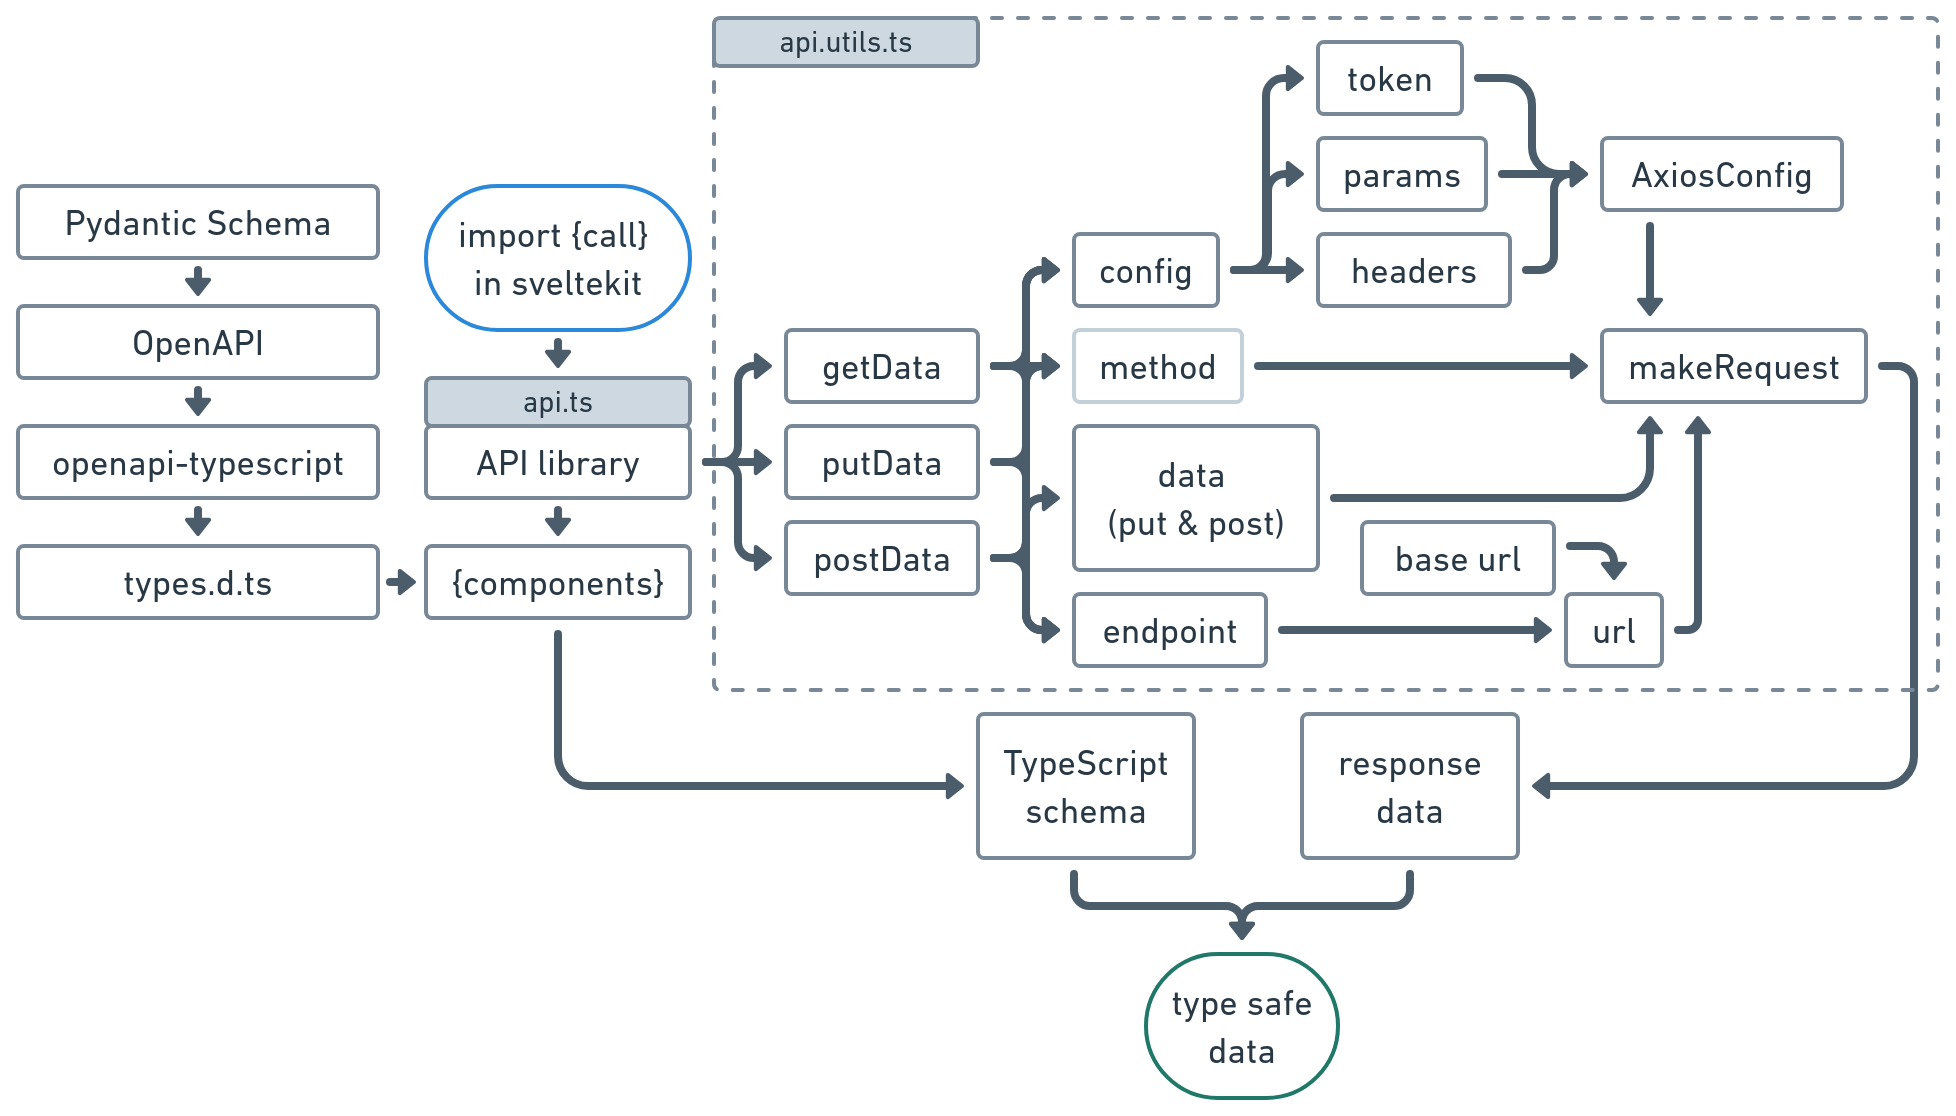
\includegraphics[width=\linewidth]{images/api-lib.png}}
\vspace{-20pt}
\caption{Custom API Client (frontend/src/lib/api*.ts)}
\label{fig:api-lib}
\vspace{-5pt}
\end{figure}

As discussed in \ref{SvelteKit}, the API is consumed by the frontend using a custom-made API client. Figure \ref{fig:api-lib} presents a more detailed view. 

\texttt{api-utils.ts} defines the abstract functions and builds the required axios configuration dynamically based on the input parameters. Strong typing is especially important here as it ensures that errors are caught early. The use of promises ensures that errors are properly propagated and can be handled by the callers of these functions.

\texttt{api.ts} defines the actual API calls for each endpoint with asynchronous functions for non-blocking execution. openapi-typescript generates a \texttt{types.d.ts} as discussed in \ref{SvelteKit}, and is combined with the response data to provide type safe data to SvelteKit.

\section{Layout}
\begin{figure}[h]
\centering
\caption{Navigation Bar (frontend/src/routes/*.*/)}
\vspace{-5pt}
\frame{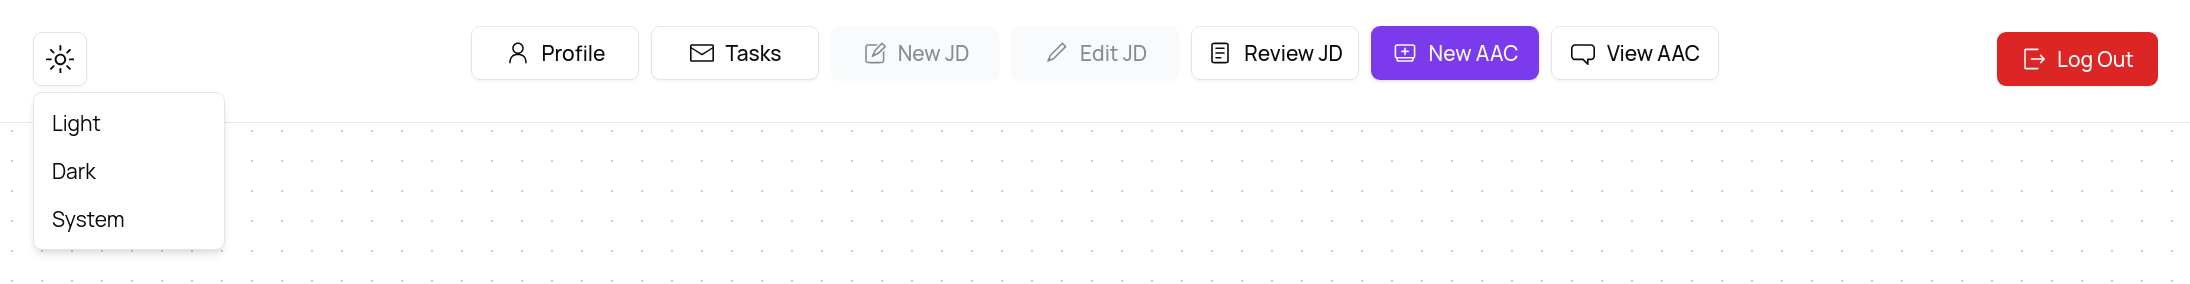
\includegraphics[width=\linewidth]{images/nav.png}}
\label{fig:nav}
\vspace{-20pt}
\end{figure}
As discussed in \ref{File Structure}, the layout is responsible for the header, body, and footer of all children. To present the correct buttons to the user in the nav-bar, a reactive store is used to keep track of the user's roles stored in the backend. If a user is not approved, but has requested a certain role, then they are still shown the button but in a greyed out format. This feedback makes the user aware of which roles they must select to gain access to specific parts of the system. The body of the page is a \texttt{<slot>} enclosed in containers that make the page fully responsive to all devices, aspect ratios, and zoom levels. It is also responsible for importing the global CSS file \texttt{app.pcss}

\section{Authentication}
Good security is essential in this process, as any bad actors could access sensitive information such as personal details, or delay recruitment by disrupting the system.

\begin{figure}[h]
\centering
\frame{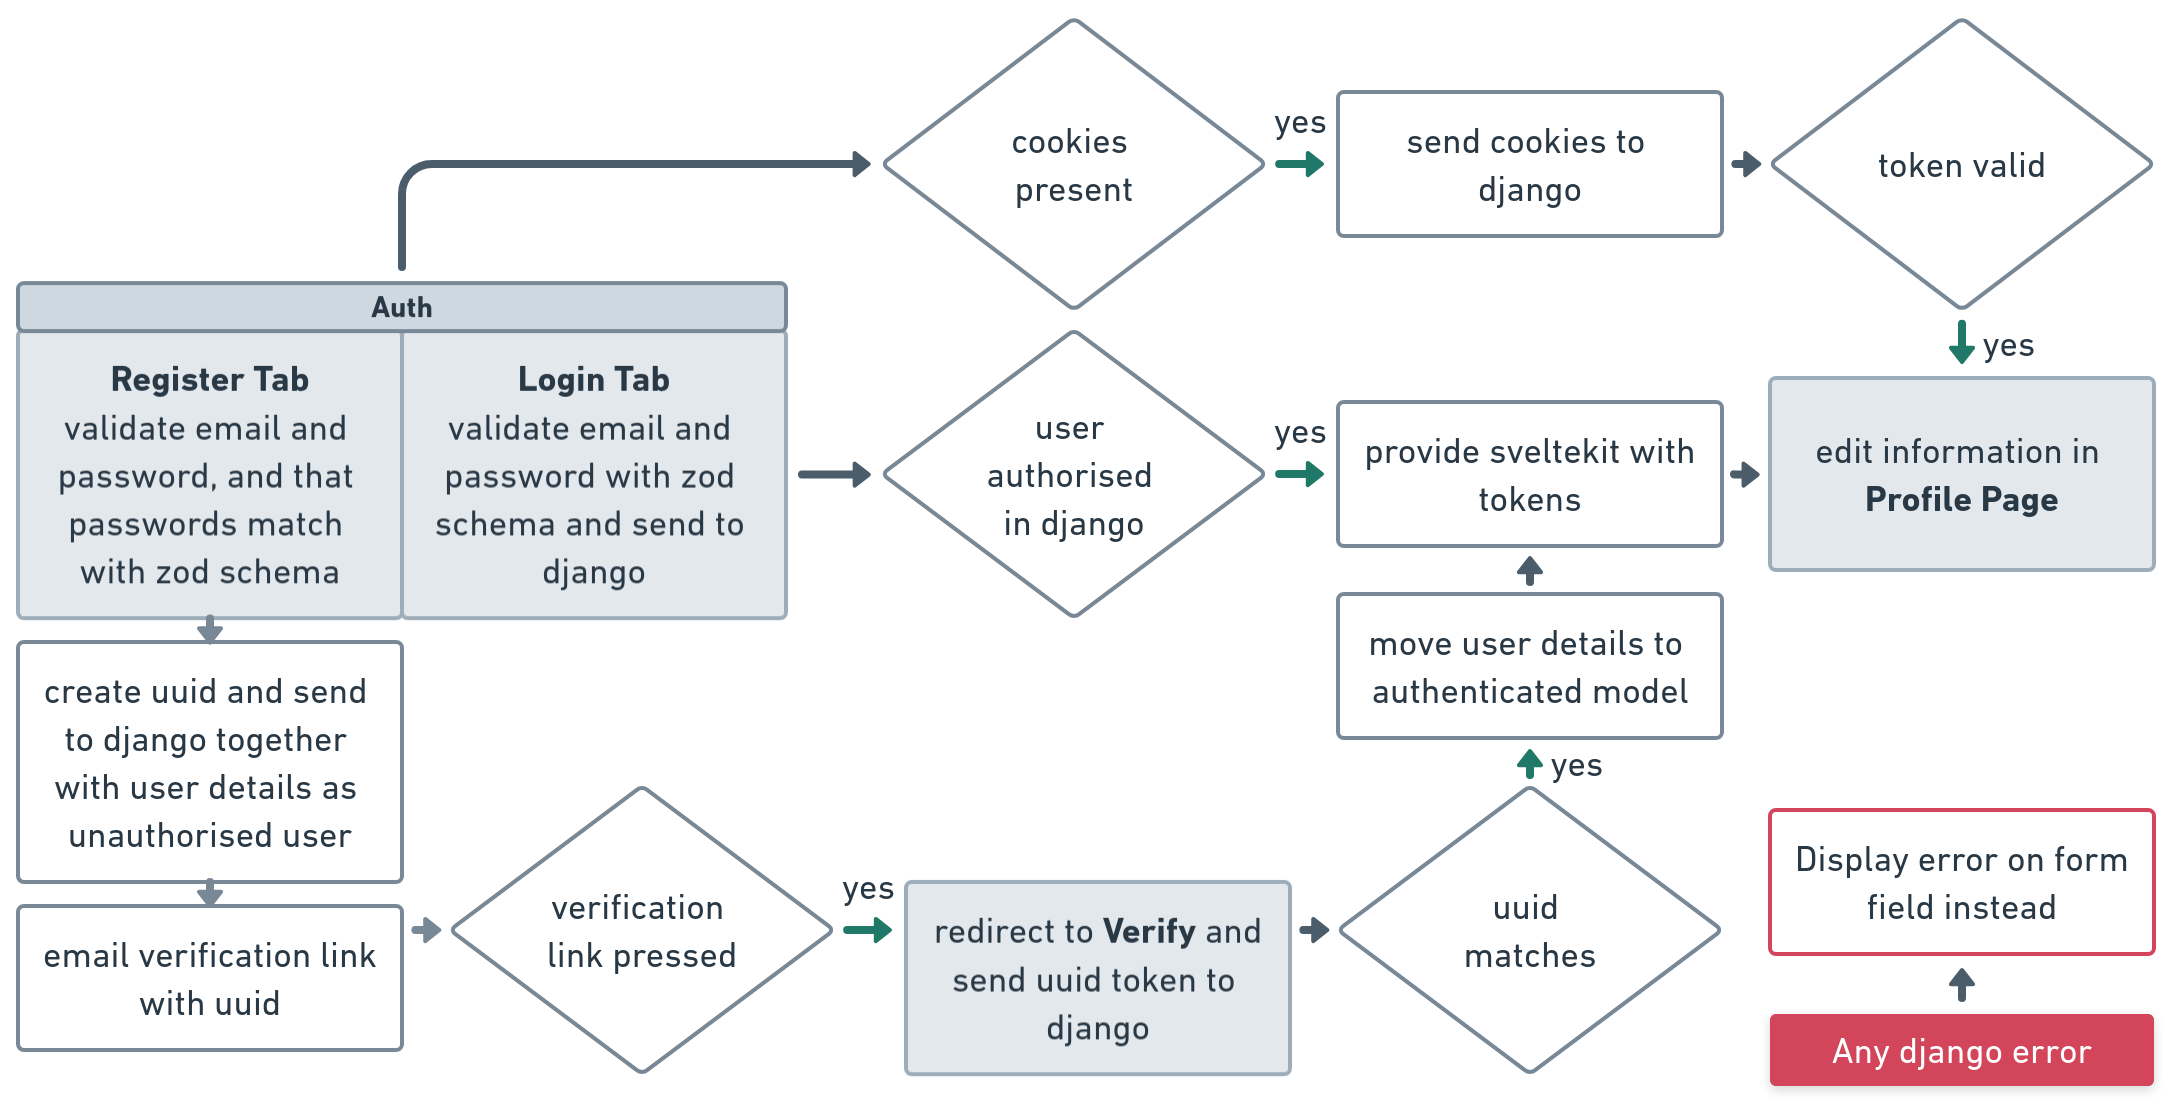
\includegraphics[width=\linewidth]{images/auth.png}}
\vspace{-20pt}
\caption{Authentication flow (frontend/src/routes/auth/*) \& (backend/users/*)}
\label{fig:auth}
\vspace{-5pt}
\end{figure}

Figure \ref{fig:auth} represents the authentication process. A high level overview has already been provided in \ref{Routes}, so this section will focus on the security steps taken. In both components, email and password is validated according to a predefined Zod schema which add a layer of data integrity and security, ensuring that the credentials meet the system's standards before being sent to Django. Screenshots of the login and registration components, along with their validation errors, can be found in Appendix \ref{app:Auth}.
\subsection{Registration}
Email verification is a necessity to ensure that users do not create fraudulent accounts. Upon registration, the system generates a universally unique identifier (UUID) token and stores it in Django's database.  It is a one-time, non-guessable token that securely links the email verification request to the user's pending account status in the database. This UUID is embedded into a link which is sent to the user's email address with Postmark. Once the link is clicked, the system verifies the token and activates the user's account.

For a more fluid user experience, this process returns a token automatically, so that the user does not have to log in manually. The token is stored in a Secure HTTP-only cookie, shielding access from client-side scripts. The HTTP-only restriction is an effective countermeasure against cross-site scripting (XSS) attacks, and the Secure flag, ensures that the cookie is only sent over HTTPS connections. A helpful addition is that the Secure flag is disabled in development mode.

Robust error handling is included to let users know why their login or registration attempts may have failed. Attempts to generate accounts with existing emails, or invalid login information is met with an immediate and clear error message. On the other hand, a successful registration attempt is met with a toast, as users require alternative positive feedback when there is no redirection.
\subsection{Login}

Users are automatically logged in as \texttt{hooks.server.ts} check whether cookies are present on every request. Otherwise the user is redirected to the auth route to log in.

\section{Profile}
\begin{figure}[h]
\centering
\frame{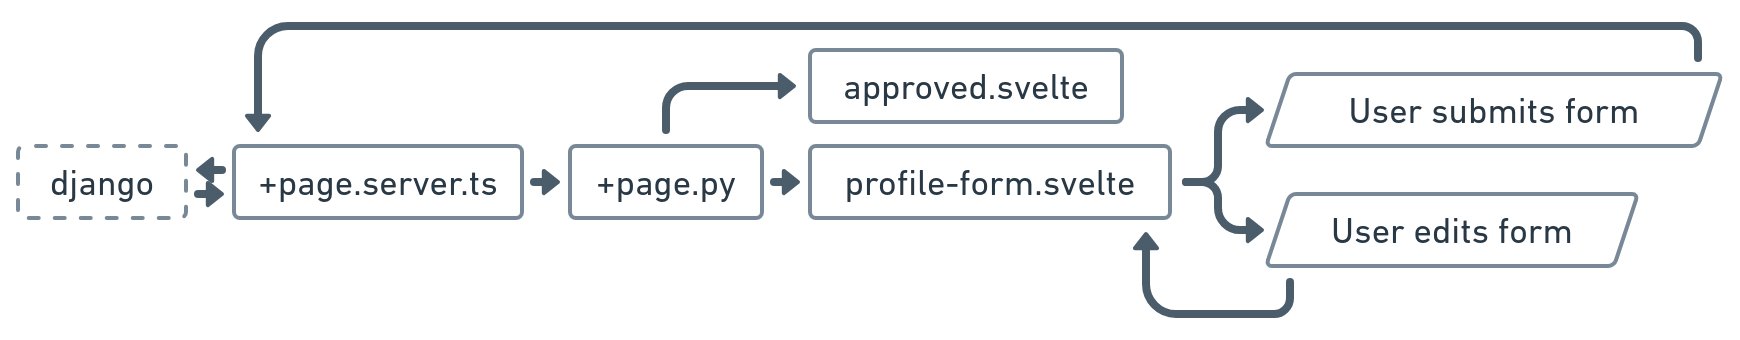
\includegraphics[width=\linewidth]{images/profile-file-flow.png}}
\vspace{-20pt}
\caption{Profile file flow (frontend/src/routes/profile/*) \& (backend/*)}
\label{fig:profile-file-flow}
\vspace{-5pt}
\end{figure}


\begin{figure}[h]
\centering
\frame{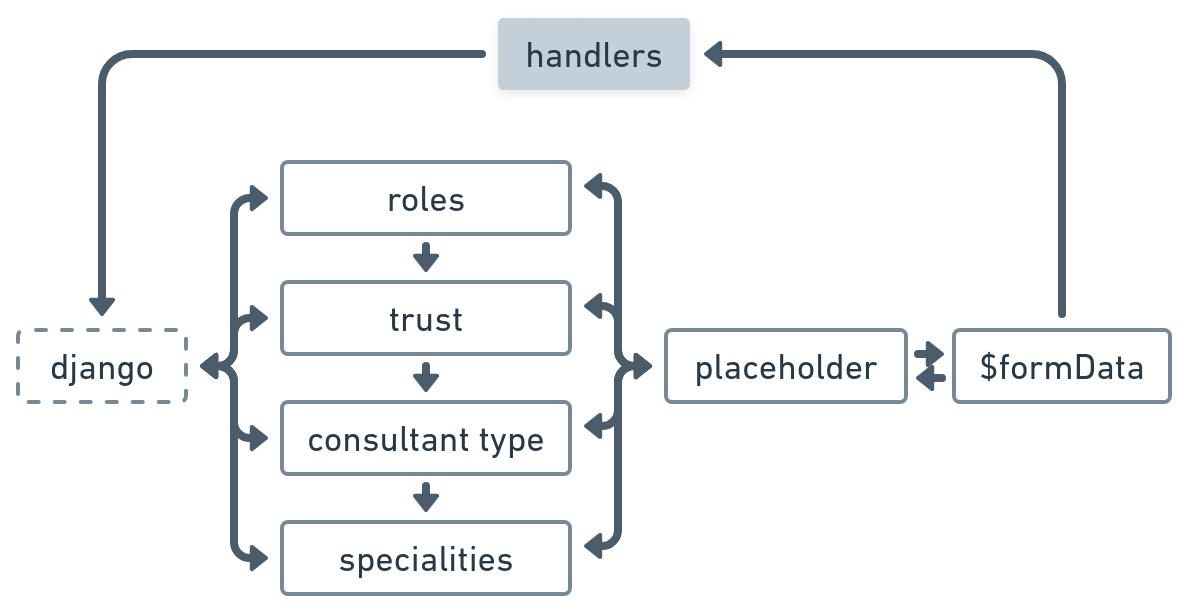
\includegraphics[width=0.65\linewidth]{images/profile-form.png}}
\vspace{-5pt}
\caption{Profile form data flow (frontend/src/routes/profile/profile-form.svelte)}
\label{fig:profile-form}
\vspace{-5pt}
\end{figure}

Figure \ref{fig:profile-file-flow} presents the exact file structure and data flow of the profile page. \texttt{approved.svelte} displays the users currently approved roles and trusts, and \texttt{profile-form.svelte} displays a form for the user to edit. A higher level explanation of this setup can be found in \ref{Routes}. 

Figure \ref{fig:profile-form} presents the data flow in the form itself. Data is initially loaded from Django, and any existing data is used as the placeholder in the field. Otherwise the user is prompted to select an item. Fields are disabled in the order in the diagram, for example, a user cannot choose a Consultant Type unless they have chosen a Role that includes one. Specialities are far more complex. For example, if a user selects Radiology, they should only be shown Specialities related to Oncology. This field must be cleared any time there is a mismatch, and requires a surprising amount of code to handle all edge cases. And there are many such edge cases, as there are multiple sources of data to be taken into account, that is the data from the page load collected from Django, the current placeholder, and the user's current selection held in \texttt{\$formData}. \texttt{profile-form.svelte} is an especially complex component as there are over 10 different placeholders that are chosen and presented dependent on a variety of factors. Screenshots of the profile page can be found in Appendix \ref{app:Profile}.

\section{Data Tables}

\section{Job Description Flow}

\section{Advisory Appointment Committees Flow}